\documentclass[Afour,times,sageh]{sagej}

\usepackage{moreverb,url,natbib, multirow, tabularx}
\usepackage[colorlinks,bookmarksopen,bookmarksnumbered,citecolor=red,urlcolor=red]{hyperref}



% tightlist command for lists without linebreak
\providecommand{\tightlist}{%
  \setlength{\itemsep}{0pt}\setlength{\parskip}{0pt}}





\begin{document}


\setcitestyle{aysep={,}}

\title{Perception of Science as a Mean to Protect the Environment}

\runninghead{Grosjean \emph{et al}.}

\author{Ph. Grosjean*\affilnum{1,2}, J. James\affilnum{2}}

\affiliation{\affilnum{1}{STAT for U, University of Mons,
Belgium}\\\affilnum{2}{Numerical Ecology Department, Complexys and
Infortech Institutes, University of Mons, Belgium}}

\corrauth{Ph. Grosjean, Numerical Ecology, University of Mons.}

\email{\href{mailto:philippe.grosjean@umons.ac.be}{\nolinkurl{philippe.grosjean@umons.ac.be}}}

\begin{abstract}
Lorem ipsum dolor sit amet, consectetur adipiscing elit. Aenean ut elit
odio. Donec fermentum tellus neque, vitae fringilla orci pretium vitae.
Fusce maximus finibus facilisis. Donec ut ullamcorper turpis. Donec ut
porta ipsum. Nullam cursus mauris a sapien ornare pulvinar. Aenean
malesuada molestie erat quis mattis. Praesent scelerisque posuere
faucibus. Praesent nunc nulla, ullamcorper ut ullamcorper sed, molestie
ut est. Donec consequat libero nisi, non semper velit vulputate et.
\end{abstract}

\keywords{survey; environment; science; perception; Germany;}

\maketitle

\hypertarget{introduction}{%
\section{Introduction}\label{introduction}}

Lorem ipsum dolor sit amet, consectetur adipiscing elit. Aenean ut elit
odio. Donec fermentum tellus neque, vitae fringilla orci pretium vitae.
Fusce maximus finibus facilisis. Donec ut ullamcorper turpis. Donec ut
porta ipsum. Nullam cursus mauris a sapien ornare pulvinar. Aenean
malesuada molestie erat quis mattis. Praesent scelerisque posuere
faucibus. Praesent nunc nulla, ullamcorper ut ullamcorper sed, molestie
ut est. Donec consequat libero nisi, non semper velit vulputate et.
Quisque eleifend tincidunt ligula, bibendum finibus massa cursus eget.
Curabitur aliquet vehicula quam non pulvinar. Aliquam facilisis tortor
nec purus finibus, sit amet elementum eros sodales. Ut porta porttitor
vestibulum. Integer molestie, leo ut maximus aliquam, velit dui iaculis
nibh, eget hendrerit purus risus sit amet dolor. Sed sed tincidunt ex.
Curabitur imperdiet egestas tellus in iaculis. Maecenas ante neque,
pretium vel nisl at, lobortis lacinia neque. In gravida elit vel
volutpat imperdiet. Sed ut nulla arcu. Proin blandit interdum ex sit
amet laoreet. Phasellus efficitur, sem hendrerit mattis dapibus, nunc
tellus ornare nisi, nec eleifend enim nibh ac ipsum. Aenean tincidunt
nisl sit amet facilisis faucibus. Donec odio erat, bibendum eu imperdiet
sed, gravida luctus turpis. Example: \citep{Taylor1937},
\citep{Knupp1999, Kamm2000}.

\hypertarget{material-and-methods}{%
\section{Material and Methods}\label{material-and-methods}}

A subpopulation of 871 people from West Germany answered to the survey
in 1993. We are particularly interested in their perception of science
in relationship with mitigation of human impact on the environment, as
in the following four questions~:

A. People believe too much in science and not enough to feelings and
faith.

B. In general, modern science is more detrimental than useful.

C. Any change in nature done by human beings risks to make things worse.

D. Modern science will solve our problems in relationship with the
environment without big changes in our way of life.

\hypertarget{results}{%
\section{Results}\label{results}}

\begin{figure}
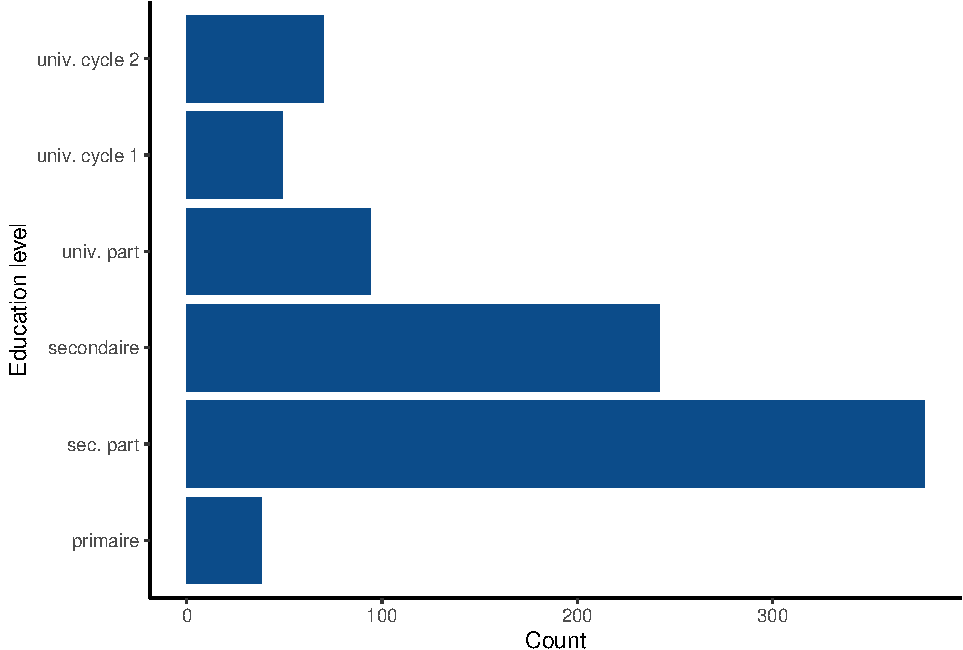
\includegraphics[width=1\linewidth]{perception_of_science_files/figure-latex/fig_edu-1} \caption{Distribution of respondants according to their education levels\label{fig:edu}.}\label{fig:fig_edu}
\end{figure}

Figure~\ref{fig:edu} presents the distribution of the sampled population
according to its education level. Quisque eleifend tincidunt ligula,
bibendum finibus massa cursus eget. Curabitur aliquet vehicula quam non
pulvinar. Aliquam facilisis tortor nec purus finibus, sit amet elementum
eros sodales. Ut porta porttitor vestibulum. Integer molestie, leo ut
maximus aliquam, velit dui iaculis nibh, eget hendrerit purus risus sit
amet dolor. Sed sed tincidunt ex. Curabitur imperdiet egestas tellus in
iaculis. Maecenas ante neque, pretium vel nisl at, lobortis lacinia
neque. In gravida elit vel volutpat imperdiet.

\hypertarget{question-b-and-education}{%
\subsection{Question B and education}\label{question-b-and-education}}

Lorem ipsum dolor sit amet, consectetur adipiscing elit. Aenean ut elit
odio. Donec fermentum tellus neque, vitae fringilla orci pretium vitae.
Fusce maximus finibus facilisis. Donec ut ullamcorper turpis. Donec ut
porta ipsum. Nullam cursus mauris a sapien ornare pulvinar. Aenean
malesuada molestie erat quis mattis. Praesent scelerisque posuere
faucibus. Praesent nunc nulla, ullamcorper ut ullamcorper sed, molestie
ut est. Donec consequat libero nisi, non semper velit vulputate et.
Quisque eleifend tincidunt ligula, bibendum finibus massa cursus eget.
Curabitur aliquet vehicula quam non pulvinar. Aliquam facilisis tortor
nec purus finibus, sit amet elementum eros sodales. Ut porta porttitor
vestibulum. Integer molestie, leo ut maximus aliquam, velit dui iaculis
nibh, eget hendrerit purus risus sit amet dolor. Sed sed tincidunt ex.
Curabitur imperdiet egestas tellus in iaculis. Maecenas ante neque,
pretium vel nisl at, lobortis lacinia neque. In gravida elit vel
volutpat imperdiet. Sed ut nulla arcu. Proin blandit interdum ex sit
amet laoreet. Phasellus efficitur, sem hendrerit mattis dapibus, nunc
tellus ornare nisi, nec eleifend enim nibh ac ipsum. Aenean tincidunt
nisl sit amet facilisis faucibus. Donec odio erat, bibendum eu imperdiet
sed, gravida luctus turpis.

Table~\ref{tab:b_edu} details the repartition of answers for question B
on whether science is more detrimental than benefic.

Lorem ipsum dolor sit amet, consectetur adipiscing elit. Aenean ut elit
odio. Donec fermentum tellus neque, vitae fringilla orci pretium vitae.
Fusce maximus finibus facilisis. Donec ut ullamcorper turpis. Donec ut
porta ipsum. Nullam cursus mauris a sapien ornare pulvinar. Aenean
malesuada molestie erat quis mattis. Praesent scelerisque posuere
faucibus. Praesent nunc nulla, ullamcorper ut ullamcorper sed, molestie
ut est. Donec consequat libero nisi, non semper velit vulputate et.
Quisque eleifend tincidunt ligula, bibendum finibus massa cursus eget.
Curabitur aliquet vehicula quam non pulvinar. Aliquam facilisis tortor
nec purus finibus, sit amet elementum eros sodales. Ut porta porttitor
vestibulum. Integer molestie, leo ut maximus aliquam, velit dui iaculis
nibh, eget hendrerit purus risus sit amet dolor. Sed sed tincidunt ex.
Curabitur imperdiet egestas tellus in iaculis. Maecenas ante neque,
pretium vel nisl at, lobortis lacinia neque. In gravida elit vel
volutpat imperdiet. Sed ut nulla arcu. Proin blandit interdum ex sit
amet laoreet. Phasellus efficitur, sem hendrerit mattis dapibus, nunc
tellus ornare nisi, nec eleifend enim nibh ac ipsum. Aenean tincidunt
nisl sit amet facilisis faucibus. Donec odio erat, bibendum eu imperdiet
sed, gravida luctus turpis.

A significant dependency between the answers to question B and the level
of education was found at \(\alpha\) level of 5\% (\(\chi^2\) test of
independence, \(\chi^2_{obs}\) = 42.76, df = 20, \emph{p}-value =
0.0022). The biplot for the first plane of a correspondance analysis
(Fig.~\ref{fig:b_edu}) shows that the lower the education, the more
respondant agree with question B

\begin{figure}
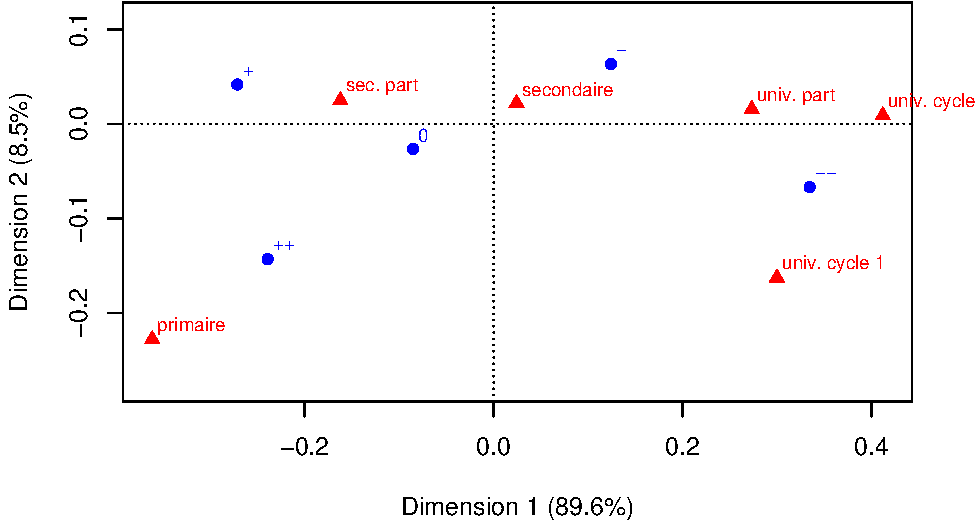
\includegraphics[width=1\linewidth]{perception_of_science_files/figure-latex/fig_b_edu-1} \caption{First plane of the correspondence analysis between answers to question B and education level\label{fig:b_edu}.}\label{fig:fig_b_edu}
\end{figure}

\hypertarget{question-d-and-education}{%
\subsection{Question D and education}\label{question-d-and-education}}

Question D is more ambiguous (Science will solve environment problems
without changing our way of life), and the answers are less clear. There
is no significant dependency at level \(\alpha\) = 5\% between answers
to question D and education level (\(\chi^2\) test of independence,
\(\chi^2_{obs}\) = 25.37, df = 20, \emph{p}-value = 0.1878).

Lorem ipsum dolor sit amet, consectetur adipiscing elit. Aenean ut elit
odio. Donec fermentum tellus neque, vitae fringilla orci pretium vitae.
Fusce maximus finibus facilisis. Donec ut ullamcorper turpis. Donec ut
porta ipsum. Nullam cursus mauris a sapien ornare pulvinar. Aenean
malesuada molestie erat quis mattis. Praesent scelerisque posuere
faucibus. Praesent nunc nulla, ullamcorper ut ullamcorper sed, molestie
ut est. Donec consequat libero nisi, non semper velit vulputate et.
Quisque eleifend tincidunt ligula, bibendum finibus massa cursus eget.
Curabitur aliquet vehicula quam non pulvinar. Aliquam facilisis tortor
nec purus finibus, sit amet elementum eros sodales. Ut porta porttitor
vestibulum. Integer molestie, leo ut maximus aliquam, velit dui iaculis
nibh, eget hendrerit purus risus sit amet dolor. Sed sed tincidunt ex.
Curabitur imperdiet egestas tellus in iaculis. Maecenas ante neque,
pretium vel nisl at, lobortis lacinia neque. In gravida elit vel
volutpat imperdiet. Sed ut nulla arcu. Proin blandit interdum ex sit
amet laoreet. Phasellus efficitur, sem hendrerit mattis dapibus, nunc
tellus ornare nisi, nec eleifend enim nibh ac ipsum. Aenean tincidunt
nisl sit amet facilisis faucibus. Donec odio erat, bibendum eu imperdiet
sed, gravida luctus turpis.

\hypertarget{discussion}{%
\section{Discussion}\label{discussion}}

Lorem ipsum dolor sit amet, consectetur adipiscing elit. Aenean ut elit
odio. Donec fermentum tellus neque, vitae fringilla orci pretium vitae.
Fusce maximus finibus facilisis. Donec ut ullamcorper turpis. Donec ut
porta ipsum. Nullam cursus mauris a sapien ornare pulvinar. Aenean
malesuada molestie erat quis mattis. Praesent scelerisque posuere
faucibus. Praesent nunc nulla, ullamcorper ut ullamcorper sed, molestie
ut est. Donec consequat libero nisi, non semper velit vulputate et.
Quisque eleifend tincidunt ligula, bibendum finibus massa cursus eget.
Curabitur aliquet vehicula quam non pulvinar. Aliquam facilisis tortor
nec purus finibus, sit amet elementum eros sodales. Ut porta porttitor
vestibulum. Integer molestie, leo ut maximus aliquam, velit dui iaculis
nibh, eget hendrerit purus risus sit amet dolor. Sed sed tincidunt ex.
Curabitur imperdiet egestas tellus in iaculis. Maecenas ante neque,
pretium vel nisl at, lobortis lacinia neque. In gravida elit vel
volutpat imperdiet. Sed ut nulla arcu. Proin blandit interdum ex sit
amet laoreet. Phasellus efficitur, sem hendrerit mattis dapibus, nunc
tellus ornare nisi, nec eleifend enim nibh ac ipsum. Aenean tincidunt
nisl sit amet facilisis faucibus. Donec odio erat, bibendum eu imperdiet
sed, gravida luctus turpis.

\hypertarget{author-contributions}{%
\section{Author Contributions}\label{author-contributions}}

Each author would like that the others have contributed more to this
manuscript!

\hypertarget{acknowledgments}{%
\section{Acknowledgments}\label{acknowledgments}}

The authors wish to thank the PerSciF FPSE UMONS for the opportunity to
submit these results.

\begin{table}[ht]
\centering
\begin{tabular}{rrrrrrr}
  \hline
 & primaire & sec. part & secondaire & univ. part & univ. cycle 1 & univ. cycle 2 \\ 
  \hline
++ &   6 &  34 &  19 &   6 &   4 &   2 \\ 
  + &  10 &  93 &  47 &  12 &   5 &   7 \\ 
  0 &  11 &  95 &  55 &  18 &  11 &  15 \\ 
  - &   7 & 112 &  82 &  37 &  16 &  27 \\ 
  -- &   4 &  44 &  39 &  21 &  13 &  19 \\ 
   \hline
\end{tabular}
\caption{Repartition of answers to question B according to education level.} 
\label{tab:b_edu}
\end{table}

\bibliographystyle{sageh}
\bibliography{bibfile}


\end{document}
